\documentclass[11pt,a4paper]{article}

% ============================================================================
% PACKAGES
% ============================================================================
\usepackage[utf8]{inputenc}
\usepackage[T1]{fontenc}
\usepackage{amsmath,amssymb,amsthm}
\usepackage{graphicx}
\usepackage{xcolor}
\usepackage{tikz}
\usetikzlibrary{shapes,arrows,positioning,fit,calc,decorations.pathreplacing,backgrounds}
\usepackage{algorithm}
\usepackage{algpseudocode}
\usepackage[margin=1in]{geometry}
\usepackage{hyperref}
\usepackage{booktabs}
\usepackage{enumitem}
\usepackage{pifont}
\usepackage{tcolorbox}
\tcbuselibrary{theorems,skins,breakable}

% ============================================================================
% CUSTOM ENVIRONMENTS
% ============================================================================
\newtcolorbox{keyinsight}{
    colback=blue!5!white,
    colframe=blue!75!black,
    fonttitle=\bfseries,
    title=Key Insight,
    breakable
}

\newtcolorbox{warningbox}{
    colback=red!5!white,
    colframe=red!75!black,
    fonttitle=\bfseries,
    title=Warning,
    breakable
}

\newtcolorbox{definitionbox}[1][]{
    colback=green!5!white,
    colframe=green!50!black,
    fonttitle=\bfseries,
    title=#1,
    breakable
}

\newtcolorbox{mathbox}[1][]{
    colback=yellow!5!white,
    colframe=orange!75!black,
    fonttitle=\bfseries,
    title=#1,
    breakable
}

\newtcolorbox{stepbox}[1][]{
    colback=purple!5!white,
    colframe=purple!60!black,
    fonttitle=\bfseries,
    title=#1,
    breakable
}

\newtcolorbox{examplebox}[1][]{
    colback=gray!5!white,
    colframe=gray!60!black,
    fonttitle=\bfseries,
    title=#1,
    breakable
}

% ============================================================================
% DOCUMENT INFO
% ============================================================================
\title{\textbf{Graph Neural Networks for Clustering Irregular Antenna Arrays}\\[0.5em]
\large A Complete Step-by-Step Guide from First Principles}
\author{Technical Reference Document}
\date{\today}

% ============================================================================
% DOCUMENT START
% ============================================================================
\begin{document}

\maketitle

\begin{abstract}
This document provides a comprehensive, step-by-step guide to clustering irregular $16 \times 16$ antenna arrays using Graph Neural Networks (GNNs). We begin with a brief explanation of why Physics-Informed Neural Networks (PINNs) are unsuitable for this task, then develop the GNN approach from absolute fundamentals---assuming no prior knowledge of graph theory or neural networks. Every concept is built incrementally with detailed explanations, visualizations, and concrete examples.
\end{abstract}

\tableofcontents
\newpage

% ============================================================================
% SECTION 1: PROBLEM DEFINITION
% ============================================================================
\section{Understanding the Problem}

\subsection{What Do We Have?}

You have a $16 \times 16$ \textbf{Uniform Rectangular Array (URA)} with \textbf{fixed inter-element spacing}. This means:
\begin{itemize}
    \item $N = 256$ individual antenna elements arranged in a perfect grid
    \item Elements are aligned horizontally and vertically (not scattered)
    \item \textbf{Fixed spacing:} $d_x$ (horizontal) and $d_y$ (vertical), typically $0.5\lambda$ or $0.7\lambda$
\end{itemize}

\begin{mathbox}[Array Geometry Definition]
The position of element $(m, n)$ where $m, n \in \{0, 1, \ldots, 15\}$ is:
\begin{equation}
\mathbf{p}_{m,n} = \begin{pmatrix} x_{m,n} \\ y_{m,n} \end{pmatrix} = \begin{pmatrix} m \cdot d_x \\ n \cdot d_y \end{pmatrix}
\end{equation}
where the horizontal and vertical spacings are \textbf{different}:
\begin{itemize}
    \item $d_x = 0.5\lambda$ (horizontal spacing between columns)
    \item $d_y = 0.7\lambda$ (vertical spacing between rows)
    \item $\lambda = c/f$ is the wavelength at operating frequency $f$
\end{itemize}
\end{mathbox}

\begin{center}
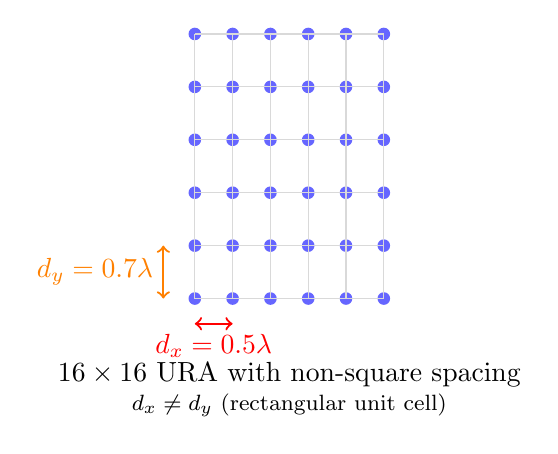
\begin{tikzpicture}[scale=0.8]
    % Draw the 6x6 subset of array with different spacing
    \foreach \x in {0,1,2,3,4,5} {
        \foreach \y in {0,1,2,3,4,5} {
            \fill[blue!60] (\x*0.6, \y*0.84) circle (0.1);
        }
    }
    
    % Spacing annotations - DIFFERENT in x and y
    \draw[<->, thick, red] (0, -0.4) -- (0.6, -0.4) node[midway, below] {$d_x = 0.5\lambda$};
    \draw[<->, thick, orange] (-0.5, 0) -- (-0.5, 0.84) node[midway, left] {$d_y = 0.7\lambda$};
    
    % Grid lines (light)
    \foreach \x in {0,1,2,3,4,5} {
        \draw[gray!30, thin] (\x*0.6, 0) -- (\x*0.6, 4.2);
    }
    \foreach \y in {0,1,2,3,4,5} {
        \draw[gray!30, thin] (0, \y*0.84) -- (3.0, \y*0.84);
    }
    
    % Labels
    \node at (1.5, -1.2) {$16 \times 16$ URA with non-square spacing};
    \node at (1.5, -1.7) {\footnotesize $d_x \neq d_y$ (rectangular unit cell)};
    
\end{tikzpicture}
\end{center}

\begin{keyinsight}
\textbf{Non-Square Unit Cell:} With $d_x = 0.5\lambda$ and $d_y = 0.7\lambda$, the array has a \textbf{rectangular} (not square) unit cell. This asymmetry affects:
\begin{itemize}
    \item Mutual coupling: horizontal neighbors are more strongly coupled than vertical
    \item Beamforming: different scan ranges in azimuth vs.\ elevation
    \item Clustering: the GNN must learn this asymmetry from the edge features
\end{itemize}
\end{keyinsight}

\subsection{Your Specific Array Configuration}

\begin{table}[h]
\centering
\caption{Array Spacing Configuration: $d_x = 0.5\lambda$, $d_y = 0.7\lambda$}
\begin{tabular}{@{}lcc@{}}
\toprule
\textbf{Parameter} & \textbf{Horizontal ($x$)} & \textbf{Vertical ($y$)} \\
\midrule
Spacing & $d_x = 0.5\lambda$ & $d_y = 0.7\lambda$ \\
Physical size (at 10 GHz) & 15 mm & 21 mm \\
Array aperture & $15 \times 0.5\lambda = 7.5\lambda$ & $15 \times 0.7\lambda = 10.5\lambda$ \\
Grating lobe onset & $\theta_x > 90°$ (none) & $\theta_y > 45°$ \\
Adjacent coupling & Strong ($\approx -10$ dB) & Moderate ($\approx -15$ dB) \\
\bottomrule
\end{tabular}
\end{table}

\begin{warningbox}
\textbf{Asymmetric Spacing Implications:}
\begin{itemize}
    \item Horizontal neighbors (same row) are \textbf{closer} ($0.5\lambda$) $\Rightarrow$ stronger mutual coupling
    \item Vertical neighbors (same column) are \textbf{farther} ($0.7\lambda$) $\Rightarrow$ weaker coupling
    \item The GNN edge features must encode this asymmetry: $(\Delta m \cdot d_x, \Delta n \cdot d_y)$
    \item Clustering may naturally favor horizontal groupings due to stronger horizontal coupling
\end{itemize}
\end{warningbox}

\subsection{What Do We Want?}

\textbf{Clustering} means partitioning the 256 grid elements into $K$ distinct groups (subarrays). For example, with $K=4$ clusters on a regular grid:

\begin{center}
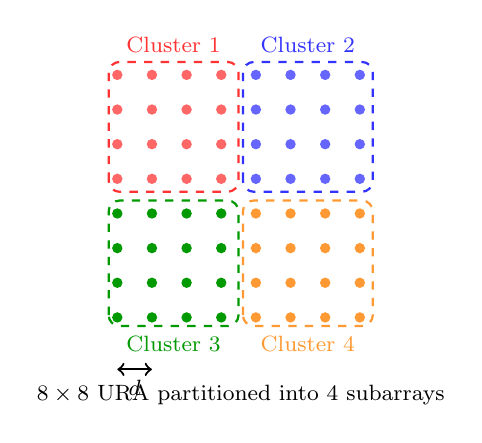
\begin{tikzpicture}[scale=0.55]
    % Draw 8x8 grid with 4 clusters (2x2 quadrants)
    
    % Cluster 1 - red (top-left quadrant)
    \foreach \x in {0,1,2,3} {
        \foreach \y in {4,5,6,7} {
            \fill[red!60] (\x*0.8, \y*0.8) circle (0.12);
        }
    }
    \draw[red!80, thick, dashed, rounded corners] (-0.2, 2.9) rectangle (2.8, 5.9);
    \node[red!80, font=\footnotesize] at (1.3, 6.3) {Cluster 1};
    
    % Cluster 2 - blue (top-right quadrant)
    \foreach \x in {4,5,6,7} {
        \foreach \y in {4,5,6,7} {
            \fill[blue!60] (\x*0.8, \y*0.8) circle (0.12);
        }
    }
    \draw[blue!80, thick, dashed, rounded corners] (2.9, 2.9) rectangle (5.9, 5.9);
    \node[blue!80, font=\footnotesize] at (4.4, 6.3) {Cluster 2};
    
    % Cluster 3 - green (bottom-left quadrant)
    \foreach \x in {0,1,2,3} {
        \foreach \y in {0,1,2,3} {
            \fill[green!60!black] (\x*0.8, \y*0.8) circle (0.12);
        }
    }
    \draw[green!60!black, thick, dashed, rounded corners] (-0.2, -0.2) rectangle (2.8, 2.7);
    \node[green!60!black, font=\footnotesize] at (1.3, -0.6) {Cluster 3};
    
    % Cluster 4 - orange (bottom-right quadrant)
    \foreach \x in {4,5,6,7} {
        \foreach \y in {0,1,2,3} {
            \fill[orange!80] (\x*0.8, \y*0.8) circle (0.12);
        }
    }
    \draw[orange!80, thick, dashed, rounded corners] (2.9, -0.2) rectangle (5.9, 2.7);
    \node[orange!80, font=\footnotesize] at (4.4, -0.6) {Cluster 4};
    
    % Spacing indicator
    \draw[<->, thick] (0, -1.2) -- (0.8, -1.2) node[midway, below, font=\footnotesize] {$d$};
    
    \node at (2.85, -1.8) {\footnotesize $8 \times 8$ URA partitioned into 4 subarrays};
\end{tikzpicture}
\hspace{1cm}
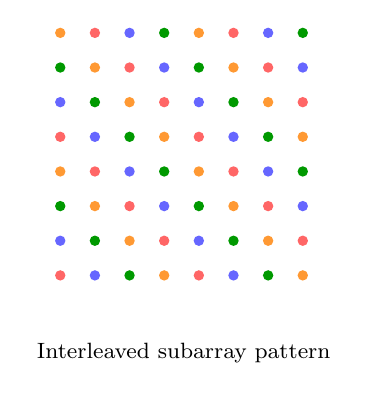
\begin{tikzpicture}[scale=0.55]
    % Alternative clustering: interleaved pattern
    
    \foreach \x in {0,1,2,3,4,5,6,7} {
        \foreach \y in {0,1,2,3,4,5,6,7} {
            \pgfmathtruncatemacro{\cluster}{mod(\x + \y, 4)}
            \ifnum\cluster=0
                \fill[red!60] (\x*0.8, \y*0.8) circle (0.12);
            \fi
            \ifnum\cluster=1
                \fill[blue!60] (\x*0.8, \y*0.8) circle (0.12);
            \fi
            \ifnum\cluster=2
                \fill[green!60!black] (\x*0.8, \y*0.8) circle (0.12);
            \fi
            \ifnum\cluster=3
                \fill[orange!80] (\x*0.8, \y*0.8) circle (0.12);
            \fi
        }
    }
    
    \node at (2.85, -1.8) {\footnotesize Interleaved subarray pattern};
\end{tikzpicture}
\end{center}

\begin{warningbox}
\textbf{The Clustering Challenge:} Even though element positions are fixed on a regular grid, finding the \textit{optimal} clustering is non-trivial because:
\begin{itemize}
    \item Mutual coupling varies across the array (edge vs.\ center elements)
    \item Different clustering patterns yield different beamforming capabilities
    \item Hardware constraints may require specific cluster shapes or sizes
    \item The number of possible partitions is astronomically large: $K^N$ for $K$ clusters
\end{itemize}
\end{warningbox}

\subsection{Why Cluster Antenna Arrays?}

Clustering serves practical purposes in antenna system design:
\begin{enumerate}
    \item \textbf{Subarraying:} Instead of controlling 256 elements individually, control $K$ groups (reduces computational complexity from $O(N)$ to $O(K)$)
    \item \textbf{Beamforming simplification:} Apply the same weights to elements in a cluster
    \item \textbf{Fault tolerance:} If one element fails, its cluster can compensate
    \item \textbf{Hardware mapping:} Assign clusters to physical processing units or RF chains
\end{enumerate}

% ============================================================================
% SECTION 2: WHY NOT PINN
% ============================================================================
\section{Why Not Use Physics-Informed Neural Networks?}

\begin{warningbox}
\textbf{Short Answer:} PINNs solve the \textit{wrong type of problem}. They are designed for differential equations, not geometric partitioning.
\end{warningbox}

\subsection{What PINNs Are Designed For}

Physics-Informed Neural Networks (PINNs) embed physical laws---typically \textbf{Partial Differential Equations (PDEs)}---into the training loss. They excel at:
\begin{itemize}
    \item Solving PDEs (heat equation, wave equation, Navier-Stokes)
    \item Discovering unknown PDE parameters from data
    \item Surrogate modeling for physical simulations
\end{itemize}

The core PINN loss function looks like:
\begin{equation}
\mathcal{L}_{\text{PINN}} = \underbrace{\|u_{\text{predicted}} - u_{\text{data}}\|^2}_{\text{data fitting}} + \lambda \underbrace{\left\| \frac{\partial^2 u}{\partial x^2} + \frac{\partial^2 u}{\partial y^2} - f \right\|^2}_{\text{PDE residual (e.g., Laplace equation)}}
\end{equation}

\subsection{Why This Fails for Clustering}

\begin{center}
\begin{tabular}{@{}p{6cm}p{6cm}@{}}
\toprule
\textbf{PINN Requirements} & \textbf{Clustering Reality} \\
\midrule
Continuous output field $u(x,y)$ & Discrete labels $\{1, 2, \ldots, K\}$ \\
Physical law as PDE & No governing PDE exists \\
Spatial derivatives $\nabla u$, $\nabla^2 u$ & Derivatives are meaningless for labels \\
Smooth solutions preferred & Cluster boundaries are discontinuous \\
\bottomrule
\end{tabular}
\end{center}

\textbf{Bottom line:} Clustering is a \textit{combinatorial optimization} problem over a \textit{discrete space}. PINNs operate in \textit{continuous function spaces} governed by \textit{differential equations}. These are fundamentally incompatible paradigms.

\vspace{1em}
\textbf{The right tool:} Graph Neural Networks naturally handle discrete structures, learn from local neighborhoods, and are designed for exactly this type of problem.

% ============================================================================
% SECTION 3: GNN FROM SCRATCH
% ============================================================================
\section{Graph Neural Networks: Building from Zero}

We will now build up the entire GNN framework step by step, assuming you have never seen a graph or neural network before.

\subsection{Step 1: What is a Graph?}

\begin{stepbox}[Step 1: Understanding Graphs]
A \textbf{graph} is a mathematical structure consisting of:
\begin{itemize}
    \item \textbf{Nodes} (also called vertices): The ``things'' we care about
    \item \textbf{Edges}: Connections between nodes
\end{itemize}
\end{stepbox}

\begin{center}
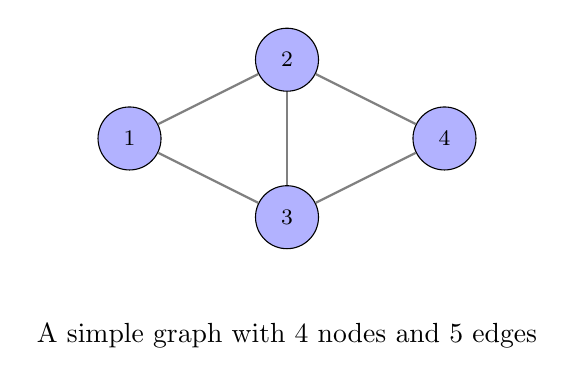
\begin{tikzpicture}[
    node/.style={circle, draw, fill=blue!30, minimum size=0.8cm, font=\footnotesize},
    edge/.style={thick, gray}
]
    \node[node] (1) at (0, 0) {1};
    \node[node] (2) at (2, 1) {2};
    \node[node] (3) at (2, -1) {3};
    \node[node] (4) at (4, 0) {4};
    
    \draw[edge] (1) -- (2);
    \draw[edge] (1) -- (3);
    \draw[edge] (2) -- (3);
    \draw[edge] (2) -- (4);
    \draw[edge] (3) -- (4);
    
    \node at (2, -2.5) {A simple graph with 4 nodes and 5 edges};
\end{tikzpicture}
\end{center}

We write this mathematically as:
\begin{align}
\mathcal{G} &= (\mathcal{V}, \mathcal{E}) \\
\mathcal{V} &= \{1, 2, 3, 4\} \quad \text{(set of nodes)} \\
\mathcal{E} &= \{(1,2), (1,3), (2,3), (2,4), (3,4)\} \quad \text{(set of edges)}
\end{align}

\subsection{Step 2: Your Antenna Array as a Graph}

\begin{stepbox}[Step 2: Converting the URA to a Graph]
Each antenna element on the grid becomes a \textbf{node}. We create \textbf{edges} based on the regular grid structure---connecting each element to its immediate neighbors.
\end{stepbox}

For your $16 \times 16$ URA with spacing $d_x$ and $d_y$:
\begin{itemize}
    \item $|\mathcal{V}| = N = 256$ nodes (one per antenna)
    \item Each node has a \textbf{feature vector} $\mathbf{x}_i$ encoding its grid position
    \item Edges follow the natural grid connectivity (4-connected or 8-connected)
\end{itemize}

\begin{definitionbox}[Node Features for Regular Grid]
For element at grid position $(m, n)$, the feature vector is:
\begin{equation}
\mathbf{x}_{m,n} = \begin{pmatrix} m \cdot d_x \\ n \cdot d_y \end{pmatrix} \in \mathbb{R}^2 \quad \text{(physical position)}
\end{equation}
Or using normalized grid indices:
\begin{equation}
\mathbf{x}_{m,n} = \begin{pmatrix} m / 15 \\ n / 15 \end{pmatrix} \in [0, 1]^2 \quad \text{(normalized indices)}
\end{equation}

We can also include additional features:
\begin{equation}
\mathbf{x}_{m,n} = \begin{pmatrix} m \cdot d_x \\ n \cdot d_y \\ \mathbb{1}_{\text{edge}}(m,n) \\ |M_{m,n}^{\text{self}}| \end{pmatrix} \in \mathbb{R}^4
\end{equation}
where $\mathbb{1}_{\text{edge}}$ indicates if the element is on the array boundary (different coupling behavior).
\end{definitionbox}

\begin{center}
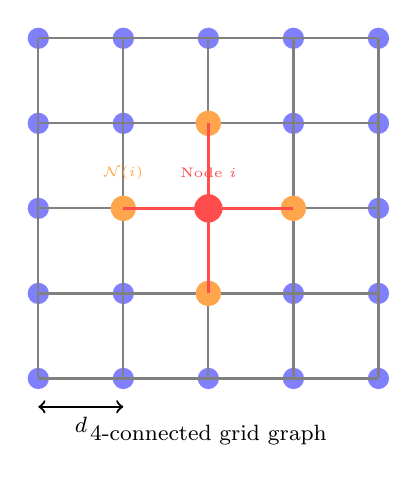
\begin{tikzpicture}[scale=0.9]
    % 5x5 grid example
    \foreach \x in {0,1,2,3,4} {
        \foreach \y in {0,1,2,3,4} {
            \fill[blue!50] (\x*1.2, \y*1.2) circle (0.15);
        }
    }
    
    % 4-connected edges (horizontal and vertical only)
    \foreach \x in {0,1,2,3,4} {
        \foreach \y in {0,1,2,3} {
            \draw[gray, thick] (\x*1.2, \y*1.2) -- (\x*1.2, \y*1.2 + 1.2);
        }
    }
    \foreach \x in {0,1,2,3} {
        \foreach \y in {0,1,2,3,4} {
            \draw[gray, thick] (\x*1.2, \y*1.2) -- (\x*1.2 + 1.2, \y*1.2);
        }
    }
    
    % Highlight one node and its neighbors
    \fill[red!70] (2.4, 2.4) circle (0.2);
    \fill[orange!70] (1.2, 2.4) circle (0.18);
    \fill[orange!70] (3.6, 2.4) circle (0.18);
    \fill[orange!70] (2.4, 1.2) circle (0.18);
    \fill[orange!70] (2.4, 3.6) circle (0.18);
    
    % Edges to neighbors highlighted
    \draw[red!70, very thick] (2.4, 2.4) -- (1.2, 2.4);
    \draw[red!70, very thick] (2.4, 2.4) -- (3.6, 2.4);
    \draw[red!70, very thick] (2.4, 2.4) -- (2.4, 1.2);
    \draw[red!70, very thick] (2.4, 2.4) -- (2.4, 3.6);
    
    % Labels
    \node[font=\footnotesize] at (2.4, -0.8) {4-connected grid graph};
    \node[font=\tiny, red!70] at (2.4, 2.9) {Node $i$};
    \node[font=\tiny, orange!70] at (1.2, 2.9) {$\mathcal{N}(i)$};
    
    % Spacing label
    \draw[<->, thick] (0, -0.4) -- (1.2, -0.4) node[midway, below, font=\footnotesize] {$d$};
    
\end{tikzpicture}
\end{center}

\subsection{Step 3: How to Create Edges}

\begin{stepbox}[Step 3: Building the Edge Set for a Regular Grid]
For a URA with fixed spacing, we leverage the natural grid structure. The connectivity pattern significantly affects clustering results.
\end{stepbox}

\subsubsection{Strategy A: 4-Connected Grid (Von Neumann Neighborhood)}

Connect each element to its 4 immediate neighbors (up, down, left, right):

\begin{mathbox}[4-Connected Edge Construction]
For element at grid position $(m, n)$:
\begin{equation}
\mathcal{N}_4(m,n) = \{(m\pm 1, n), (m, n\pm 1)\} \cap \{0, \ldots, 15\}^2
\end{equation}
\textbf{Properties:}
\begin{itemize}
    \item Interior elements: 4 neighbors
    \item Edge elements: 3 neighbors  
    \item Corner elements: 2 neighbors
    \item Total edges: $|\mathcal{E}| = 2 \times 16 \times 15 = 480$
\end{itemize}
\end{mathbox}

\subsubsection{Strategy B: 8-Connected Grid (Moore Neighborhood)}

Include diagonal neighbors as well:

\begin{mathbox}[8-Connected Edge Construction]
\begin{equation}
\mathcal{N}_8(m,n) = \{(m+\Delta m, n+\Delta n) : \Delta m, \Delta n \in \{-1, 0, 1\}, (\Delta m, \Delta n) \neq (0,0)\}
\end{equation}
\textbf{Properties:}
\begin{itemize}
    \item Interior elements: 8 neighbors
    \item More connectivity $\Rightarrow$ information flows faster through the GNN
    \item Diagonal edges have distance $\sqrt{2} \cdot d$ (useful for edge features)
\end{itemize}
\end{mathbox}

\begin{center}
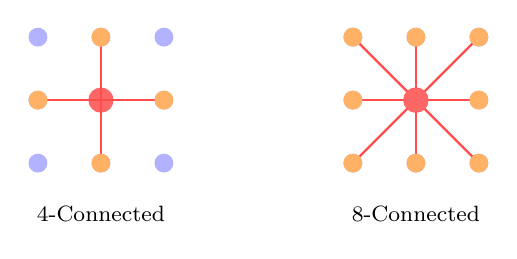
\begin{tikzpicture}[scale=0.8]
    % 4-connected
    \begin{scope}[xshift=0cm]
        \foreach \x in {0,1,2} {
            \foreach \y in {0,1,2} {
                \fill[blue!30] (\x, \y) circle (0.15);
            }
        }
        \fill[red!60] (1, 1) circle (0.2);
        
        % 4 edges
        \draw[thick, red!70] (1,1) -- (0,1);
        \draw[thick, red!70] (1,1) -- (2,1);
        \draw[thick, red!70] (1,1) -- (1,0);
        \draw[thick, red!70] (1,1) -- (1,2);
        
        \fill[orange!60] (0,1) circle (0.15);
        \fill[orange!60] (2,1) circle (0.15);
        \fill[orange!60] (1,0) circle (0.15);
        \fill[orange!60] (1,2) circle (0.15);
        
        \node at (1, -0.8) {\footnotesize 4-Connected};
    \end{scope}
    
    % 8-connected
    \begin{scope}[xshift=5cm]
        \foreach \x in {0,1,2} {
            \foreach \y in {0,1,2} {
                \fill[blue!30] (\x, \y) circle (0.15);
            }
        }
        \fill[red!60] (1, 1) circle (0.2);
        
        % 8 edges
        \draw[thick, red!70] (1,1) -- (0,1);
        \draw[thick, red!70] (1,1) -- (2,1);
        \draw[thick, red!70] (1,1) -- (1,0);
        \draw[thick, red!70] (1,1) -- (1,2);
        \draw[thick, red!70] (1,1) -- (0,0);
        \draw[thick, red!70] (1,1) -- (2,0);
        \draw[thick, red!70] (1,1) -- (0,2);
        \draw[thick, red!70] (1,1) -- (2,2);
        
        \foreach \x in {0,1,2} {
            \foreach \y in {0,1,2} {
                \fill[orange!60] (\x, \y) circle (0.15);
            }
        }
        \fill[red!60] (1, 1) circle (0.2);
        
        \node at (1, -0.8) {\footnotesize 8-Connected};
    \end{scope}
\end{tikzpicture}
\end{center}

\subsubsection{Strategy C: Extended Neighborhood (for Larger Receptive Field)}

Connect to neighbors within $r$ grid steps:
\begin{equation}
\mathcal{N}_r(m,n) = \{(m', n') : |m - m'| \leq r \text{ and } |n - n'| \leq r\} \setminus \{(m,n)\}
\end{equation}

\subsubsection{Strategy D: Mutual Coupling-Based Edges}

Connect elements with strong electromagnetic coupling:
\begin{equation}
\mathcal{E}_{\text{coupling}} = \{((m,n), (m',n')) : |M_{(m,n),(m',n')}| > \tau\}
\end{equation}
This can be combined with grid-based edges to incorporate physics.

\begin{keyinsight}
\textbf{Recommendation for $16 \times 16$ URA:} Start with \textbf{8-connected} grid edges. This provides good local connectivity while respecting the regular structure. Add coupling-based edges if EM simulation data is available.
\end{keyinsight}

\subsection{Step 4: The Adjacency Matrix}

\begin{stepbox}[Step 4: Matrix Representation of Graphs]
For computation, we represent the graph as an \textbf{adjacency matrix} $\mathbf{A} \in \mathbb{R}^{N \times N}$.
\end{stepbox}

\begin{mathbox}[Adjacency Matrix Definition]
\begin{equation}
A_{ij} = \begin{cases}
1 & \text{if edge } (i,j) \in \mathcal{E} \\
0 & \text{otherwise}
\end{cases}
\end{equation}
\end{mathbox}

\begin{examplebox}[Example: Adjacency Matrix]
For the 4-node graph from Step 1:
\begin{equation}
\mathbf{A} = \begin{pmatrix}
0 & 1 & 1 & 0 \\
1 & 0 & 1 & 1 \\
1 & 1 & 0 & 1 \\
0 & 1 & 1 & 0
\end{pmatrix}
\end{equation}
Row $i$, column $j$: is there an edge from $i$ to $j$?
\end{examplebox}

We also define the \textbf{degree matrix}:
\begin{equation}
D_{ii} = \sum_{j=1}^{N} A_{ij} = \text{number of neighbors of node } i
\end{equation}

\subsection{Step 5: What is a Neural Network? (Brief Review)}

\begin{stepbox}[Step 5: Neural Network Basics]
A neural network is a function $f_\theta$ that transforms inputs to outputs through layers of linear transformations and non-linear activations.
\end{stepbox}

A single layer:
\begin{equation}
\mathbf{h} = \sigma(\mathbf{W}\mathbf{x} + \mathbf{b})
\end{equation}
where:
\begin{itemize}
    \item $\mathbf{x} \in \mathbb{R}^{d_{\text{in}}}$: input vector
    \item $\mathbf{W} \in \mathbb{R}^{d_{\text{out}} \times d_{\text{in}}}$: learnable weight matrix
    \item $\mathbf{b} \in \mathbb{R}^{d_{\text{out}}}$: learnable bias vector
    \item $\sigma$: non-linear activation function (e.g., ReLU, tanh)
    \item $\mathbf{h} \in \mathbb{R}^{d_{\text{out}}}$: output vector
\end{itemize}

\begin{center}
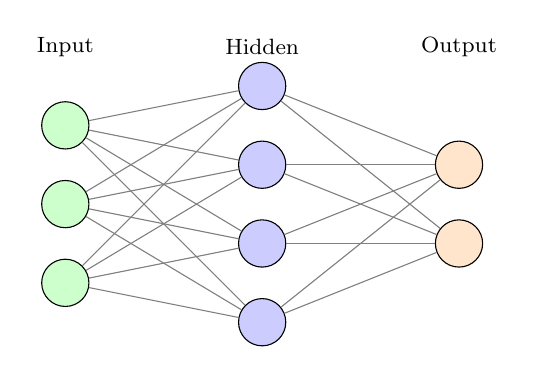
\begin{tikzpicture}[
    neuron/.style={circle, draw, minimum size=0.6cm},
    arrow/.style={->, thick}
]
    % Input layer
    \foreach \i in {1,2,3} {
        \node[neuron, fill=green!20] (i\i) at (0, -\i) {};
    }
    \node at (0, 0) {\footnotesize Input};
    
    % Hidden layer
    \foreach \i in {1,2,3,4} {
        \node[neuron, fill=blue!20] (h\i) at (2.5, -\i + 0.5) {};
    }
    \node at (2.5, 0) {\footnotesize Hidden};
    
    % Output layer
    \foreach \i in {1,2} {
        \node[neuron, fill=orange!20] (o\i) at (5, -\i - 0.5) {};
    }
    \node at (5, 0) {\footnotesize Output};
    
    % Connections
    \foreach \i in {1,2,3} {
        \foreach \j in {1,2,3,4} {
            \draw[gray, thin] (i\i) -- (h\j);
        }
    }
    \foreach \i in {1,2,3,4} {
        \foreach \j in {1,2} {
            \draw[gray, thin] (h\i) -- (o\j);
        }
    }
\end{tikzpicture}
\end{center}

\subsection{Step 6: The Key Idea of GNNs---Message Passing}

\begin{stepbox}[Step 6: Message Passing (The Core Concept)]
In a regular neural network, each input is processed independently. In a GNN, each node \textbf{aggregates information from its neighbors} to update its representation. This is called \textbf{message passing}.
\end{stepbox}

\begin{keyinsight}
The fundamental insight: \textit{A node's representation should depend on its neighbors.} In antenna arrays, this means: an element's cluster assignment should be influenced by the elements around it.
\end{keyinsight}

The general message passing formula for one layer:

\begin{mathbox}[Message Passing Equation]
\begin{equation}
\boxed{
\mathbf{h}_i^{(\ell+1)} = \text{UPDATE}\left( \mathbf{h}_i^{(\ell)}, \text{AGGREGATE}\left( \left\{ \mathbf{h}_j^{(\ell)} : j \in \mathcal{N}(i) \right\} \right) \right)
}
\end{equation}
where:
\begin{itemize}
    \item $\mathbf{h}_i^{(\ell)}$: representation (embedding) of node $i$ at layer $\ell$
    \item $\mathcal{N}(i)$: the neighbors of node $i$ (nodes connected by an edge)
    \item AGGREGATE: combines neighbor information (sum, mean, max, attention)
    \item UPDATE: combines self-information with aggregated neighbor information
\end{itemize}
\end{mathbox}

\begin{center}
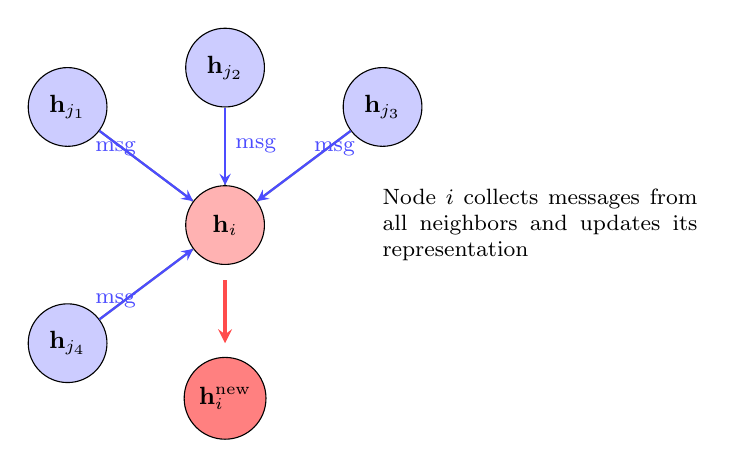
\begin{tikzpicture}[
    node/.style={circle, draw, minimum size=1cm, font=\small},
    arrow/.style={->, thick, >=stealth}
]
    % Central node
    \node[node, fill=red!30] (center) at (0, 0) {$\mathbf{h}_i$};
    
    % Neighbors
    \node[node, fill=blue!20] (n1) at (-2, 1.5) {$\mathbf{h}_{j_1}$};
    \node[node, fill=blue!20] (n2) at (0, 2) {$\mathbf{h}_{j_2}$};
    \node[node, fill=blue!20] (n3) at (2, 1.5) {$\mathbf{h}_{j_3}$};
    \node[node, fill=blue!20] (n4) at (-2, -1.5) {$\mathbf{h}_{j_4}$};
    
    % Edges
    \draw[thick, gray] (center) -- (n1);
    \draw[thick, gray] (center) -- (n2);
    \draw[thick, gray] (center) -- (n3);
    \draw[thick, gray] (center) -- (n4);
    
    % Messages
    \draw[arrow, blue!70] (n1) -- (center) node[midway, above left, font=\footnotesize] {msg};
    \draw[arrow, blue!70] (n2) -- (center) node[midway, right, font=\footnotesize] {msg};
    \draw[arrow, blue!70] (n3) -- (center) node[midway, above right, font=\footnotesize] {msg};
    \draw[arrow, blue!70] (n4) -- (center) node[midway, below left, font=\footnotesize] {msg};
    
    % Updated node
    \draw[arrow, very thick, red!70] (0, -0.7) -- (0, -1.5);
    \node[node, fill=red!50] (updated) at (0, -2.2) {$\mathbf{h}_i^{\text{new}}$};
    
    \node at (4, 0) {\parbox{4cm}{\footnotesize Node $i$ collects messages from all neighbors and updates its representation}};
\end{tikzpicture}
\end{center}

\subsection{Step 7: A Concrete GNN Layer---Graph Convolutional Network (GCN)}

\begin{stepbox}[Step 7: The GCN Layer]
The Graph Convolutional Network (GCN) is the simplest and most foundational GNN architecture.
\end{stepbox}

\begin{mathbox}[GCN Layer Equation]
\begin{equation}
\mathbf{H}^{(\ell+1)} = \sigma\left( \tilde{\mathbf{D}}^{-1/2} \tilde{\mathbf{A}} \tilde{\mathbf{D}}^{-1/2} \mathbf{H}^{(\ell)} \mathbf{W}^{(\ell)} \right)
\end{equation}
Let's break this down piece by piece:
\begin{itemize}
    \item $\tilde{\mathbf{A}} = \mathbf{A} + \mathbf{I}$: adjacency matrix with self-loops added
    \item $\tilde{\mathbf{D}}$: degree matrix of $\tilde{\mathbf{A}}$
    \item $\tilde{\mathbf{D}}^{-1/2} \tilde{\mathbf{A}} \tilde{\mathbf{D}}^{-1/2}$: normalized adjacency (prevents exploding/vanishing values)
    \item $\mathbf{H}^{(\ell)} \in \mathbb{R}^{N \times d_\ell}$: all node embeddings at layer $\ell$
    \item $\mathbf{W}^{(\ell)} \in \mathbb{R}^{d_\ell \times d_{\ell+1}}$: learnable weight matrix
    \item $\sigma$: activation function (ReLU or similar)
\end{itemize}
\end{mathbox}

\textbf{What does this actually do?} For a single node $i$:
\begin{equation}
\mathbf{h}_i^{(\ell+1)} = \sigma\left( \mathbf{W}^{(\ell)\top} \cdot \sum_{j \in \mathcal{N}(i) \cup \{i\}} \frac{\mathbf{h}_j^{(\ell)}}{\sqrt{|\mathcal{N}(i)| \cdot |\mathcal{N}(j)|}} \right)
\end{equation}

In plain English: \textit{``Average your neighbors' features (including yourself), transform with a learned matrix, apply non-linearity.''}

\subsection{Step 8: Graph Attention Networks (GAT)---Learning Which Neighbors Matter}

\begin{stepbox}[Step 8: Attention Mechanism]
GCN treats all neighbors equally. But some neighbors are more important than others! GAT learns \textbf{attention weights} to focus on relevant neighbors.
\end{stepbox}

\begin{mathbox}[GAT Layer Equations]
\textbf{Step 8.1:} Compute attention coefficients between node $i$ and neighbor $j$:
\begin{equation}
e_{ij} = \text{LeakyReLU}\left( \mathbf{a}^\top \left[ \mathbf{W}\mathbf{h}_i \,\|\, \mathbf{W}\mathbf{h}_j \right] \right)
\end{equation}
where $\|$ denotes concatenation, $\mathbf{a}$ is a learnable attention vector.

\textbf{Step 8.2:} Normalize with softmax over neighbors:
\begin{equation}
\alpha_{ij} = \frac{\exp(e_{ij})}{\sum_{k \in \mathcal{N}(i)} \exp(e_{ik})}
\end{equation}
Now $\sum_{j \in \mathcal{N}(i)} \alpha_{ij} = 1$.

\textbf{Step 8.3:} Update node representation:
\begin{equation}
\mathbf{h}_i^{(\ell+1)} = \sigma\left( \sum_{j \in \mathcal{N}(i)} \alpha_{ij} \mathbf{W} \mathbf{h}_j^{(\ell)} \right)
\end{equation}
\end{mathbox}

\begin{center}
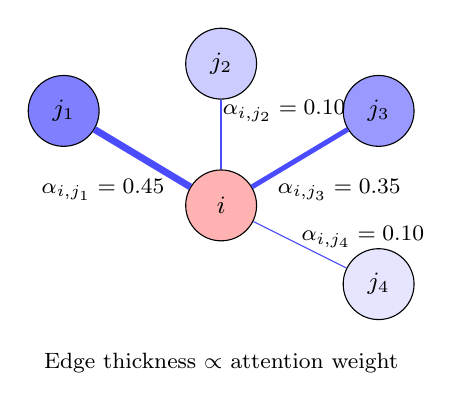
\begin{tikzpicture}[
    node/.style={circle, draw, minimum size=0.9cm, font=\small},
    arrow/.style={->, thick, >=stealth}
]
    % Central node
    \node[node, fill=red!30] (center) at (0, 0) {$i$};
    
    % Neighbors with different attention
    \node[node, fill=blue!50] (n1) at (-2, 1.2) {$j_1$};
    \node[node, fill=blue!20] (n2) at (0, 1.8) {$j_2$};
    \node[node, fill=blue!40] (n3) at (2, 1.2) {$j_3$};
    \node[node, fill=blue!10] (n4) at (2, -1) {$j_4$};
    
    % Edges with varying thickness (attention)
    \draw[line width=2.5pt, blue!70] (n1) -- (center);
    \draw[line width=0.8pt, blue!70] (n2) -- (center);
    \draw[line width=1.8pt, blue!70] (n3) -- (center);
    \draw[line width=0.4pt, blue!70] (n4) -- (center);
    
    % Attention labels
    \node[font=\footnotesize] at (-1.5, 0.2) {$\alpha_{i,j_1}=0.45$};
    \node[font=\footnotesize] at (0.8, 1.2) {$\alpha_{i,j_2}=0.10$};
    \node[font=\footnotesize] at (1.5, 0.2) {$\alpha_{i,j_3}=0.35$};
    \node[font=\footnotesize] at (1.8, -0.4) {$\alpha_{i,j_4}=0.10$};
    
    \node at (0, -2) {\footnotesize Edge thickness $\propto$ attention weight};
\end{tikzpicture}
\end{center}

\textbf{Multi-head attention:} Run $K$ independent attention mechanisms and concatenate:
\begin{equation}
\mathbf{h}_i^{(\ell+1)} = \Big\|_{k=1}^{K} \sigma\left( \sum_{j \in \mathcal{N}(i)} \alpha_{ij}^{(k)} \mathbf{W}^{(k)} \mathbf{h}_j^{(\ell)} \right)
\end{equation}

\subsection{Step 9: Edge Features---Incorporating Physics}

\begin{stepbox}[Step 9: Adding Edge Information for Fixed-Spacing Arrays]
For a URA with fixed spacing $d \in \{0.5\lambda, 0.7\lambda\}$, edge features encode the \textbf{relative position} and \textbf{electromagnetic coupling} between connected elements.
\end{stepbox}

\begin{mathbox}[Physics-Informed Edge Features for Asymmetric URA]
For edge between elements $(m_1, n_1)$ and $(m_2, n_2)$ with $d_x = 0.5\lambda$, $d_y = 0.7\lambda$:
\begin{equation}
\mathbf{e}_{(m_1,n_1) \to (m_2,n_2)} = \begin{pmatrix}
\Delta x / \lambda \\[0.3em]
\Delta y / \lambda \\[0.3em]
r / \lambda \\[0.3em]
|M_{ij}| \\[0.3em]
\angle M_{ij}
\end{pmatrix} = \begin{pmatrix}
(m_2 - m_1) \cdot 0.5 \\[0.3em]
(n_2 - n_1) \cdot 0.7 \\[0.3em]
\sqrt{(\Delta m \cdot 0.5)^2 + (\Delta n \cdot 0.7)^2} \\[0.3em]
\text{Mutual coupling magnitude} \\[0.3em]
\text{Mutual coupling phase}
\end{pmatrix}
\end{equation}

\textbf{Key insight:} Horizontal neighbor $(\Delta m = 1, \Delta n = 0)$ has distance $0.5\lambda$, while vertical neighbor $(\Delta m = 0, \Delta n = 1)$ has distance $0.7\lambda$. The GNN learns to treat these differently!
\end{mathbox}

\subsubsection{Mutual Coupling in URAs}

For a URA with spacing $d$, the mutual coupling between elements depends primarily on their separation:

\begin{mathbox}[Mutual Coupling Model]
For two elements separated by distance $r_{ij}$:
\begin{equation}
M_{ij} \approx \frac{e^{-jkr_{ij}}}{r_{ij}} \cdot f(\theta_{ij}, \phi_{ij})
\end{equation}
where:
\begin{itemize}
    \item $k = 2\pi/\lambda$ is the wavenumber
    \item $r_{ij} = d \cdot \sqrt{(\Delta m)^2 + (\Delta n)^2}$ for grid offset $(\Delta m, \Delta n)$
    \item $f(\theta, \phi)$ accounts for element pattern and polarization
\end{itemize}

\textbf{Key insight:} Elements at the same grid distance have similar (but not identical) coupling due to edge effects.
\end{mathbox}

\subsubsection{Edge Features by Neighbor Type}

\begin{table}[h]
\centering
\caption{Coupling Characteristics for $d_x = 0.5\lambda$, $d_y = 0.7\lambda$}
\begin{tabular}{@{}lccc@{}}
\toprule
\textbf{Neighbor Type} & \textbf{Distance} & \textbf{Coupling} & \textbf{Edge Feature $r/\lambda$} \\
\midrule
Horizontal ($\Delta m = \pm 1$) & $0.5\lambda$ & Strong ($\approx -10$ dB) & 0.5 \\
Vertical ($\Delta n = \pm 1$) & $0.7\lambda$ & Moderate ($\approx -15$ dB) & 0.7 \\
Diagonal ($|\Delta m| = |\Delta n| = 1$) & $0.86\lambda$ & Weak ($\approx -20$ dB) & $\sqrt{0.5^2 + 0.7^2} \approx 0.86$ \\
\bottomrule
\end{tabular}
\end{table}

\begin{keyinsight}
\textbf{Asymmetry Impact:} Because $d_x < d_y$, horizontal neighbors are more strongly coupled than vertical neighbors. The GNN will learn:
\begin{itemize}
    \item Elements in the same row have stronger relationships
    \item Clustering may favor ``horizontal strips'' over ``vertical strips''
    \item Diagonal connections are weaker than both horizontal and vertical
\end{itemize}
\end{keyinsight}

The GNN learns to weight these edge features appropriately during training.

\textbf{Modified message passing with edge features:}
\begin{equation}
\mathbf{h}_i^{(\ell+1)} = \sigma\left( \sum_{j \in \mathcal{N}(i)} \alpha_{ij} \cdot \text{MLP}\left( \left[ \mathbf{W}\mathbf{h}_j^{(\ell)} \,\|\, \mathbf{e}_{ij} \right] \right) \right)
\end{equation}

This allows the network to learn patterns like:
\begin{itemize}
    \item ``Strongly coupled elements should cluster together''
    \item ``Horizontal neighbors behave differently from diagonal neighbors''
    \item ``Edge elements have different coupling patterns than center elements''
\end{itemize}

\subsection{Step 10: From Node Embeddings to Cluster Assignments}

\begin{stepbox}[Step 10: The Output Layer]
After $L$ GNN layers, each node has a rich embedding $\mathbf{h}_i^{(L)} \in \mathbb{R}^{d_L}$. Now we must convert this to a cluster assignment.
\end{stepbox}

\begin{mathbox}[Soft Cluster Assignment]
Apply a final linear layer + softmax to get cluster probabilities:
\begin{equation}
\mathbf{z}_i = \text{softmax}\left( \mathbf{W}_{\text{out}} \mathbf{h}_i^{(L)} + \mathbf{b}_{\text{out}} \right) \in \mathbb{R}^K
\end{equation}
where:
\begin{itemize}
    \item $\mathbf{W}_{\text{out}} \in \mathbb{R}^{K \times d_L}$: output weight matrix
    \item $\mathbf{z}_i = (z_{i1}, z_{i2}, \ldots, z_{iK})$: probability distribution over $K$ clusters
    \item $z_{ik} = P(\text{node } i \text{ belongs to cluster } k)$
    \item $\sum_{k=1}^{K} z_{ik} = 1$ (guaranteed by softmax)
\end{itemize}
\end{mathbox}

We collect all assignments into a matrix:
\begin{equation}
\mathbf{Z} = \begin{pmatrix}
z_{11} & z_{12} & \cdots & z_{1K} \\
z_{21} & z_{22} & \cdots & z_{2K} \\
\vdots & \vdots & \ddots & \vdots \\
z_{N1} & z_{N2} & \cdots & z_{NK}
\end{pmatrix} \in \mathbb{R}^{N \times K}
\end{equation}

Row $i$ is the cluster probability distribution for antenna $i$.

\subsection{Step 11: The Loss Function---How Do We Train Without Labels?}

\begin{stepbox}[Step 11: Unsupervised Clustering Loss]
In \textbf{unsupervised} clustering, we have no ground truth labels. We must design a loss function that encourages ``good'' clusters based on the graph structure alone.
\end{stepbox}

The key principle: \textbf{good clusters minimize edges cut between them.}

\begin{center}
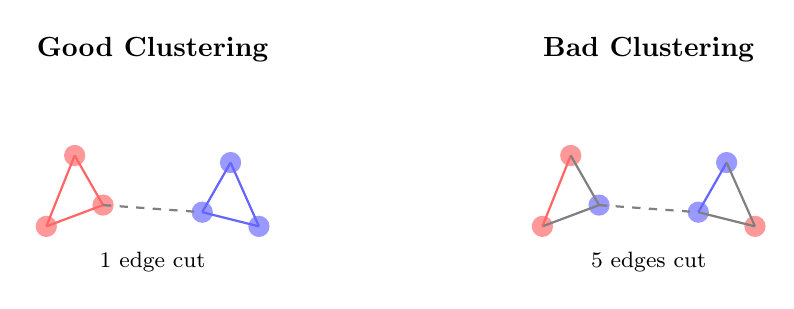
\begin{tikzpicture}[scale=0.9]
    % Good clustering
    \begin{scope}[xshift=-4cm]
        \node[font=\bfseries] at (1.5, 2.5) {Good Clustering};
        
        % Cluster 1
        \fill[red!40] (0, 0) circle (0.15);
        \fill[red!40] (0.8, 0.3) circle (0.15);
        \fill[red!40] (0.4, 1.0) circle (0.15);
        \draw[red!60, thick] (0,0) -- (0.8, 0.3);
        \draw[red!60, thick] (0,0) -- (0.4, 1.0);
        \draw[red!60, thick] (0.8, 0.3) -- (0.4, 1.0);
        
        % Cluster 2
        \fill[blue!40] (2.2, 0.2) circle (0.15);
        \fill[blue!40] (3.0, 0) circle (0.15);
        \fill[blue!40] (2.6, 0.9) circle (0.15);
        \draw[blue!60, thick] (2.2, 0.2) -- (3.0, 0);
        \draw[blue!60, thick] (2.2, 0.2) -- (2.6, 0.9);
        \draw[blue!60, thick] (3.0, 0) -- (2.6, 0.9);
        
        % Cut edge
        \draw[gray, dashed, thick] (0.8, 0.3) -- (2.2, 0.2);
        \node[font=\footnotesize] at (1.5, -0.5) {1 edge cut};
    \end{scope}
    
    % Bad clustering
    \begin{scope}[xshift=3cm]
        \node[font=\bfseries] at (1.5, 2.5) {Bad Clustering};
        
        % Mixed cluster 1
        \fill[red!40] (0, 0) circle (0.15);
        \fill[blue!40] (0.8, 0.3) circle (0.15);
        \fill[red!40] (0.4, 1.0) circle (0.15);
        \draw[gray, thick] (0,0) -- (0.8, 0.3);
        \draw[red!60, thick] (0,0) -- (0.4, 1.0);
        \draw[gray, thick] (0.8, 0.3) -- (0.4, 1.0);
        
        % Mixed cluster 2
        \fill[blue!40] (2.2, 0.2) circle (0.15);
        \fill[red!40] (3.0, 0) circle (0.15);
        \fill[blue!40] (2.6, 0.9) circle (0.15);
        \draw[gray, thick] (2.2, 0.2) -- (3.0, 0);
        \draw[blue!60, thick] (2.2, 0.2) -- (2.6, 0.9);
        \draw[gray, thick] (3.0, 0) -- (2.6, 0.9);
        
        % Cut edge
        \draw[gray, dashed, thick] (0.8, 0.3) -- (2.2, 0.2);
        \node[font=\footnotesize] at (1.5, -0.5) {5 edges cut};
    \end{scope}
\end{tikzpicture}
\end{center}

\subsubsection{Loss Component 1: MinCut Loss}

The \textbf{normalized cut} measures how many edges cross cluster boundaries:

\begin{mathbox}[MinCut Loss]
\begin{equation}
\mathcal{L}_{\text{cut}} = -\frac{\text{Tr}(\mathbf{Z}^\top \mathbf{A} \mathbf{Z})}{\text{Tr}(\mathbf{Z}^\top \mathbf{D} \mathbf{Z})}
\end{equation}
\textbf{Intuition:}
\begin{itemize}
    \item $\mathbf{Z}^\top \mathbf{A} \mathbf{Z}$: measures edges \textit{within} clusters (we want this HIGH)
    \item $\mathbf{Z}^\top \mathbf{D} \mathbf{Z}$: normalization by cluster sizes
    \item Negative sign: we minimize the loss, so we maximize within-cluster edges
\end{itemize}
\end{mathbox}

\textbf{Detailed derivation:}
\begin{align}
(\mathbf{Z}^\top \mathbf{A} \mathbf{Z})_{kk} &= \sum_{i=1}^{N} \sum_{j=1}^{N} z_{ik} \cdot A_{ij} \cdot z_{jk} \\
&= \sum_{\text{edge } (i,j)} z_{ik} \cdot z_{jk} \\
&= \text{``soft count'' of edges where both endpoints are in cluster } k
\end{align}

\subsubsection{Loss Component 2: Orthogonality Loss}

Prevent the trivial solution where all nodes go to one cluster:

\begin{mathbox}[Orthogonality Loss]
\begin{equation}
\mathcal{L}_{\text{ortho}} = \left\| \frac{\mathbf{Z}^\top \mathbf{Z}}{N} - \frac{\mathbf{I}_K}{K} \right\|_F^2
\end{equation}
\textbf{Intuition:}
\begin{itemize}
    \item $\mathbf{Z}^\top \mathbf{Z} \in \mathbb{R}^{K \times K}$: measures cluster overlap
    \item We want $\mathbf{Z}^\top \mathbf{Z} \approx \frac{N}{K} \mathbf{I}_K$ (diagonal, equal sizes)
    \item This encourages balanced, non-overlapping clusters
\end{itemize}
\end{mathbox}

\subsubsection{Loss Component 3: Entropy Regularization (Optional)}

Encourage confident (non-uniform) assignments:
\begin{equation}
\mathcal{L}_{\text{entropy}} = -\frac{1}{N} \sum_{i=1}^{N} \sum_{k=1}^{K} z_{ik} \log(z_{ik} + \epsilon)
\end{equation}
Low entropy = confident predictions (one $z_{ik}$ close to 1, others close to 0).

\subsubsection{Total Loss Function}

\begin{mathbox}[Complete Loss Function]
\begin{equation}
\boxed{
\mathcal{L}_{\text{total}} = \mathcal{L}_{\text{cut}} + \lambda_1 \mathcal{L}_{\text{ortho}} + \lambda_2 \mathcal{L}_{\text{entropy}}
}
\end{equation}
Typical values: $\lambda_1 = 1.0$, $\lambda_2 = 0.1$
\end{mathbox}

\subsection{Step 12: Complete Architecture Summary}

\begin{stepbox}[Step 12: Putting It All Together]
Here is the complete GNN architecture for antenna array clustering:
\end{stepbox}

\begin{center}
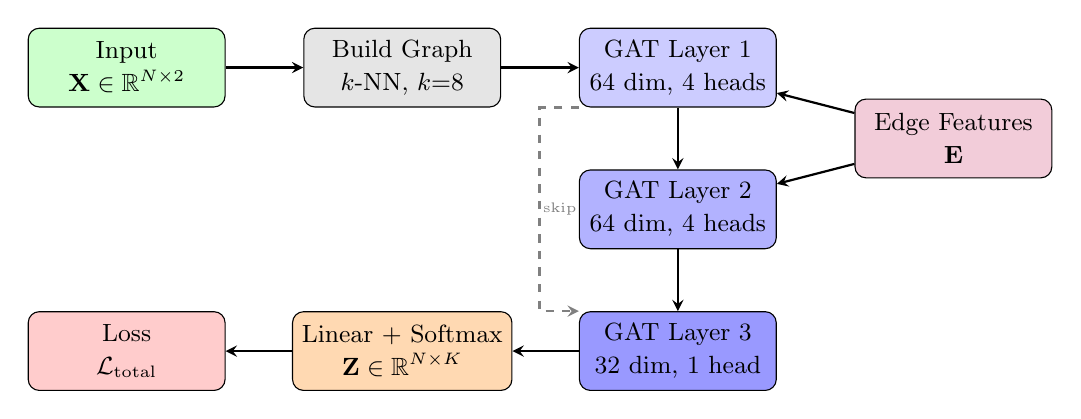
\begin{tikzpicture}[
    block/.style={rectangle, draw, rounded corners, minimum height=1cm, minimum width=2.5cm, font=\small, align=center},
    arrow/.style={->, thick, >=stealth}
]
    % Input
    \node[block, fill=green!20] (input) at (0, 0) {Input\\[0.1em]$\mathbf{X} \in \mathbb{R}^{N \times 2}$};
    
    % Graph construction
    \node[block, fill=gray!20] (graph) at (3.5, 0) {Build Graph\\[0.1em]$k$-NN, $k{=}8$};
    
    % GAT layers
    \node[block, fill=blue!20] (gat1) at (7, 0) {GAT Layer 1\\[0.1em]64 dim, 4 heads};
    \node[block, fill=blue!30] (gat2) at (7, -1.8) {GAT Layer 2\\[0.1em]64 dim, 4 heads};
    \node[block, fill=blue!40] (gat3) at (7, -3.6) {GAT Layer 3\\[0.1em]32 dim, 1 head};
    
    % Output
    \node[block, fill=orange!30] (mlp) at (3.5, -3.6) {Linear + Softmax\\[0.1em]$\mathbf{Z} \in \mathbb{R}^{N \times K}$};
    
    % Loss
    \node[block, fill=red!20] (loss) at (0, -3.6) {Loss\\[0.1em]$\mathcal{L}_{\text{total}}$};
    
    % Edge features
    \node[block, fill=purple!20] (edge) at (10.5, -0.9) {Edge Features\\[0.1em]$\mathbf{E}$};
    
    % Arrows
    \draw[arrow] (input) -- (graph);
    \draw[arrow] (graph) -- (gat1);
    \draw[arrow] (gat1) -- (gat2);
    \draw[arrow] (gat2) -- (gat3);
    \draw[arrow] (gat3) -- (mlp);
    \draw[arrow] (mlp) -- (loss);
    
    \draw[arrow] (edge) -- (gat1);
    \draw[arrow] (edge) -- (gat2);
    
    % Skip connection
    \draw[arrow, dashed, gray] (gat1.south west) -- ++(-0.5, 0) |- (gat3.north west);
    \node[font=\tiny, gray] at (5.5, -1.8) {skip};
    
\end{tikzpicture}
\end{center}

\textbf{Layer-by-layer breakdown:}
\begin{enumerate}
    \item \textbf{Input:} Antenna positions $\mathbf{X} \in \mathbb{R}^{256 \times 2}$
    \item \textbf{Graph Construction:} Build $k$-NN graph ($k=8$), compute edge features
    \item \textbf{GAT Layer 1:} $2 \to 64$ dimensions, 4 attention heads, output: $\mathbb{R}^{256 \times 256}$
    \item \textbf{GAT Layer 2:} $256 \to 64$ dimensions, 4 attention heads, output: $\mathbb{R}^{256 \times 256}$
    \item \textbf{GAT Layer 3:} $256 \to 32$ dimensions, 1 attention head, output: $\mathbb{R}^{256 \times 32}$
    \item \textbf{Output Layer:} Linear $32 \to K$ + Softmax, output: $\mathbb{R}^{256 \times K}$
\end{enumerate}

\subsection{Step 13: Training Algorithm}

\begin{stepbox}[Step 13: How to Train the Network]
\end{stepbox}

\begin{algorithm}[H]
\caption{GNN Training for Antenna Array Clustering}
\begin{algorithmic}[1]
\Require Positions $\mathbf{P} \in \mathbb{R}^{N \times 2}$, mutual coupling $\mathbf{M}$ (optional), clusters $K$
\Ensure Trained model, cluster assignments

\State \textbf{// Step A: Preprocessing}
\State Normalize positions: $\mathbf{P} \leftarrow (\mathbf{P} - \mu) / \sigma$
\State Build $k$-NN graph: $\mathcal{E} \leftarrow \text{kNN}(\mathbf{P}, k=8)$
\State Compute adjacency $\mathbf{A}$ and degree $\mathbf{D}$
\State Compute edge features: $\mathbf{e}_{ij} \leftarrow [d_{ij}, |M_{ij}|, \ldots]$ for $(i,j) \in \mathcal{E}$

\State
\State \textbf{// Step B: Initialize Network}
\State Initialize GAT layers with Xavier/Glorot initialization
\State Set learning rate $\eta = 0.001$, weight decay $= 0.0005$

\State
\State \textbf{// Step C: Training Loop}
\For{epoch $= 1$ to 500}
    \State \textbf{// Forward pass}
    \State $\mathbf{H}^{(0)} \leftarrow \mathbf{P}$
    \For{$\ell = 1$ to $L$}
        \State $\mathbf{H}^{(\ell)} \leftarrow \text{GATLayer}_\ell(\mathbf{H}^{(\ell-1)}, \mathbf{A}, \mathbf{E})$
        \State $\mathbf{H}^{(\ell)} \leftarrow \text{ELU}(\mathbf{H}^{(\ell)})$ \Comment{Activation}
        \State $\mathbf{H}^{(\ell)} \leftarrow \text{Dropout}(\mathbf{H}^{(\ell)}, p=0.1)$ \Comment{Regularization}
    \EndFor
    \State $\mathbf{Z} \leftarrow \text{Softmax}(\text{Linear}(\mathbf{H}^{(L)}))$
    
    \State
    \State \textbf{// Compute loss}
    \State $\mathcal{L}_{\text{cut}} \leftarrow -\text{Tr}(\mathbf{Z}^\top \mathbf{A} \mathbf{Z}) / \text{Tr}(\mathbf{Z}^\top \mathbf{D} \mathbf{Z})$
    \State $\mathcal{L}_{\text{ortho}} \leftarrow \|\mathbf{Z}^\top \mathbf{Z}/N - \mathbf{I}_K/K\|_F^2$
    \State $\mathcal{L} \leftarrow \mathcal{L}_{\text{cut}} + \lambda_1 \mathcal{L}_{\text{ortho}}$
    
    \State
    \State \textbf{// Backward pass}
    \State $\nabla_\Theta \mathcal{L} \leftarrow \text{Backpropagation}(\mathcal{L})$
    \State $\Theta \leftarrow \Theta - \eta \cdot \text{Adam}(\nabla_\Theta \mathcal{L})$
\EndFor

\State
\State \textbf{// Step D: Extract Final Clusters}
\State $c_i \leftarrow \arg\max_k z_{ik}$ for all $i = 1, \ldots, N$
\State \Return cluster assignments $\{c_1, c_2, \ldots, c_N\}$
\end{algorithmic}
\end{algorithm}

\subsection{Step 14: From Soft to Hard Assignments}

\begin{stepbox}[Step 14: Final Cluster Assignment]
The network outputs soft probabilities. For the final clustering, we take the hard assignment:
\end{stepbox}

\begin{equation}
c_i = \arg\max_{k \in \{1, \ldots, K\}} z_{ik}
\end{equation}

\begin{examplebox}[Example]
If node 42 has $\mathbf{z}_{42} = (0.05, 0.82, 0.08, 0.05)$ for $K=4$ clusters:
\begin{equation}
c_{42} = \arg\max(0.05, 0.82, 0.08, 0.05) = 2
\end{equation}
Antenna element 42 is assigned to Cluster 2.
\end{examplebox}

% ============================================================================
% SECTION 4: IMPLEMENTATION
% ============================================================================
\section{Implementation Guide}

\subsection{Recommended Libraries}

\begin{itemize}
    \item \textbf{PyTorch Geometric (PyG):} Most popular GNN library
    \begin{verbatim}
    pip install torch-geometric
    \end{verbatim}
    
    \item \textbf{Deep Graph Library (DGL):} Alternative, good for large graphs
    \begin{verbatim}
    pip install dgl
    \end{verbatim}
\end{itemize}

\subsection{Complete PyTorch Geometric Code}

\begin{verbatim}
import torch
import torch.nn as nn
import torch.nn.functional as F
from torch_geometric.nn import GATConv
from torch_geometric.data import Data
import numpy as np

# =============================================================
# ARRAY CONFIGURATION
# =============================================================
class URAConfig:
    """Configuration for Uniform Rectangular Array with asymmetric spacing."""
    def __init__(self, rows=16, cols=16, dx=0.5, dy=0.7, freq_ghz=10.0):
        self.rows = rows
        self.cols = cols
        self.N = rows * cols  # Total elements: 256
        # ASYMMETRIC SPACING: dx != dy
        self.dx = dx  # Horizontal spacing = 0.5 lambda
        self.dy = dy  # Vertical spacing = 0.7 lambda
        self.freq = freq_ghz * 1e9
        self.c = 3e8
        self.wavelength = self.c / self.freq
        self.dx_meters = dx * self.wavelength  # 15 mm at 10 GHz
        self.dy_meters = dy * self.wavelength  # 21 mm at 10 GHz

# =============================================================
# GRAPH CONSTRUCTION FOR REGULAR GRID
# =============================================================
def create_ura_graph(config, connectivity='8-connected'):
    """
    Create graph from URA with ASYMMETRIC spacing (dx != dy).
    
    Args:
        config: URAConfig with dx=0.5, dy=0.7
        connectivity: '4-connected' or '8-connected'
    
    Returns:
        positions: (N, 2) tensor of physical positions in wavelengths
        edge_index: (2, E) tensor of edges
        edge_attr: (E, num_features) edge features with PHYSICAL distances
    """
    rows, cols = config.rows, config.cols
    dx, dy = config.dx, config.dy  # 0.5 and 0.7 lambda
    
    # Generate grid positions with DIFFERENT spacing in x and y
    m_indices = torch.arange(cols).float()
    n_indices = torch.arange(rows).float()
    mm, nn = torch.meshgrid(m_indices, n_indices, indexing='xy')
    
    # Physical positions (asymmetric!)
    positions = torch.stack([
        mm.flatten() * dx,  # x: 0, 0.5, 1.0, 1.5, ... (in lambda)
        nn.flatten() * dy   # y: 0, 0.7, 1.4, 2.1, ... (in lambda)
    ], dim=1)  # Shape: (N, 2)
    
    # Build edges with PHYSICAL distance features
    edges = []
    edge_features = []
    
    for m in range(cols):
        for n in range(rows):
            idx = n * cols + m
            
            if connectivity == '4-connected':
                offsets = [(1, 0), (-1, 0), (0, 1), (0, -1)]
            else:  # 8-connected
                offsets = [(dm, dn) for dm in [-1, 0, 1] 
                           for dn in [-1, 0, 1] if (dm, dn) != (0, 0)]
            
            for dm, dn in offsets:
                m2, n2 = m + dm, n + dn
                if 0 <= m2 < cols and 0 <= n2 < rows:
                    idx2 = n2 * cols + m2
                    edges.append([idx, idx2])
                    
                    # Edge features with ACTUAL physical distances
                    delta_x = dm * dx  # Physical x-offset (in lambda)
                    delta_y = dn * dy  # Physical y-offset (in lambda)
                    phys_dist = np.sqrt(delta_x**2 + delta_y**2)
                    
                    # Features: [dx_physical, dy_physical, total_distance]
                    edge_features.append([delta_x, delta_y, phys_dist])
    
    edge_index = torch.tensor(edges, dtype=torch.long).T
    edge_attr = torch.tensor(edge_features, dtype=torch.float)
    
    return positions, edge_index, edge_attr


# =============================================================
# GNN MODEL
# =============================================================
class URAClusteringGNN(nn.Module):
    def __init__(self, in_dim=2, hidden_dim=64, 
                 num_clusters=4, heads=4, dropout=0.1, 
                 edge_dim=3):
        super().__init__()
        
        # Input projection
        self.input_proj = nn.Linear(in_dim, hidden_dim)
        
        # GAT layers with edge features
        self.conv1 = GATConv(hidden_dim, hidden_dim, heads=heads,
                             dropout=dropout, edge_dim=edge_dim)
        self.conv2 = GATConv(hidden_dim * heads, hidden_dim, heads=heads,
                             dropout=dropout, edge_dim=edge_dim)
        self.conv3 = GATConv(hidden_dim * heads, hidden_dim, heads=1,
                             dropout=dropout, edge_dim=edge_dim)
        
        # Output layer
        self.classifier = nn.Linear(hidden_dim, num_clusters)
        self.dropout = dropout
        
    def forward(self, x, edge_index, edge_attr):
        # Project input features
        h = F.elu(self.input_proj(x))
        
        # GNN layers
        h = F.elu(self.conv1(h, edge_index, edge_attr))
        h = F.dropout(h, p=self.dropout, training=self.training)
        
        h = F.elu(self.conv2(h, edge_index, edge_attr))
        h = F.dropout(h, p=self.dropout, training=self.training)
        
        h = self.conv3(h, edge_index, edge_attr)
        
        # Soft cluster assignments
        z = F.softmax(self.classifier(h), dim=-1)
        return z


# =============================================================
# LOSS FUNCTIONS
# =============================================================
def mincut_loss(z, adj, deg):
    """Normalized MinCut loss for graph clustering."""
    num = torch.trace(z.T @ adj @ z)
    denom = torch.trace(z.T @ deg @ z)
    return -num / (denom + 1e-8)

def orthogonality_loss(z):
    """Encourage balanced, non-overlapping clusters."""
    n, k = z.shape
    identity = torch.eye(k, device=z.device) / k
    cluster_sim = (z.T @ z) / n
    return torch.norm(cluster_sim - identity, p='fro') ** 2


# =============================================================
# TRAINING
# =============================================================
def train_ura_clustering(config, num_clusters=4, epochs=500, lr=0.001):
    """
    Train GNN for URA clustering.
    
    Args:
        config: URAConfig with spacing parameters
        num_clusters: K clusters
        epochs: training iterations
        lr: learning rate
    
    Returns:
        cluster_assignments: (N,) array of cluster labels
    """
    device = torch.device('cuda' if torch.cuda.is_available() 
                          else 'cpu')
    
    # Create graph from URA configuration
    positions, edge_index, edge_attr = create_ura_graph(
        config, connectivity='8-connected'
    )
    
    # Normalize positions to [0, 1]
    positions = (positions - positions.min(0)[0]) / \
                (positions.max(0)[0] - positions.min(0)[0])
    
    # Move to device
    positions = positions.to(device)
    edge_index = edge_index.to(device)
    edge_attr = edge_attr.to(device)
    
    # Build adjacency matrix for loss computation
    n = config.N
    adj = torch.zeros(n, n, device=device)
    adj[edge_index[0], edge_index[1]] = 1
    deg = torch.diag(adj.sum(dim=1))
    
    # Initialize model
    model = URAClusteringGNN(
        in_dim=2,
        hidden_dim=64,
        num_clusters=num_clusters,
        heads=4,
        edge_dim=edge_attr.shape[1]
    ).to(device)
    
    optimizer = torch.optim.Adam(model.parameters(), lr=lr,
                                  weight_decay=5e-4)
    
    # Training loop
    model.train()
    for epoch in range(epochs):
        optimizer.zero_grad()
        
        z = model(positions, edge_index, edge_attr)
        
        loss_cut = mincut_loss(z, adj, deg)
        loss_ortho = orthogonality_loss(z)
        loss = loss_cut + 1.0 * loss_ortho
        
        loss.backward()
        optimizer.step()
        
        if (epoch + 1) % 100 == 0:
            print(f"Epoch {epoch+1}: Loss={loss.item():.4f}")
    
    # Extract clusters
    model.eval()
    with torch.no_grad():
        z = model(positions, edge_index, edge_attr)
        clusters = z.argmax(dim=1).cpu().numpy()
    
    return clusters


# =============================================================
# EXAMPLE USAGE
# =============================================================
if __name__ == "__main__":
    # Your specific configuration: dx=0.5lambda, dy=0.7lambda
    config = URAConfig(
        rows=16, 
        cols=16, 
        dx=0.5,  # Horizontal: 0.5 lambda (closer, stronger coupling)
        dy=0.7   # Vertical: 0.7 lambda (farther, weaker coupling)
    )
    
    print(f"Array size: {config.N} elements ({config.rows}x{config.cols})")
    print(f"Horizontal spacing: {config.dx} lambda = {config.dx_meters*1000:.1f} mm")
    print(f"Vertical spacing: {config.dy} lambda = {config.dy_meters*1000:.1f} mm")
    print(f"Array aperture: {(config.cols-1)*config.dx:.1f} x "
          f"{(config.rows-1)*config.dy:.1f} lambda")
    
    # Train clustering
    clusters = train_ura_clustering(config, num_clusters=4, epochs=400)
    print(f"\nCluster sizes: {np.bincount(clusters)}")
    
    # Reshape to visualize on grid
    cluster_grid = clusters.reshape(config.rows, config.cols)
    print(f"\nCluster assignment grid (first 4 rows):")
    print(cluster_grid[:4, :])
\end{verbatim}

\subsection{Hyperparameter Recommendations}

\begin{table}[h]
\centering
\caption{Recommended Hyperparameters for $16 \times 16$ URA with $d_x = 0.5\lambda$, $d_y = 0.7\lambda$}
\begin{tabular}{@{}llp{5.5cm}@{}}
\toprule
\textbf{Parameter} & \textbf{Value} & \textbf{Reasoning} \\
\midrule
\multicolumn{3}{@{}l}{\textit{Array Configuration (Fixed)}} \\
Horizontal spacing $d_x$ & $0.5\lambda$ & Closer spacing, stronger coupling \\
Vertical spacing $d_y$ & $0.7\lambda$ & Wider spacing, weaker coupling \\
Grid connectivity & 8-connected & Captures all neighbor relationships \\
\midrule
\multicolumn{3}{@{}l}{\textit{GNN Architecture}} \\
Hidden dim & 64--128 & Sufficient for 256 elements \\
GAT heads & 4--8 & Multi-head attention for diverse patterns \\
Layers & 2--3 & 2 layers $\Rightarrow$ 2-hop neighborhood \\
Edge features & 3 & $[\Delta x, \Delta y, r]$ in wavelengths \\
\midrule
\multicolumn{3}{@{}l}{\textit{Training}} \\
Learning rate & $10^{-3}$ & Standard for Adam optimizer \\
Weight decay & $5 \times 10^{-4}$ & Regularization \\
Dropout & 0.1 & Mild regularization \\
Epochs & 300--500 & Until loss stabilizes \\
$\lambda_{\text{ortho}}$ & 1.0 & Equal weight to balance \\
\bottomrule
\end{tabular}
\end{table}

\begin{keyinsight}
\textbf{Asymmetric Spacing Impact on Clustering:}
\begin{itemize}
    \item Horizontal neighbors ($0.5\lambda$ apart) are more strongly coupled $\Rightarrow$ GNN may prefer horizontal groupings
    \item Vertical neighbors ($0.7\lambda$ apart) are more weakly coupled $\Rightarrow$ easier to ``cut'' vertically
    \item For balanced clusters, the orthogonality loss counteracts this natural bias
\end{itemize}
\end{keyinsight}

% ============================================================================
% SECTION 5: SUMMARY
% ============================================================================
\section{Summary: The Complete Pipeline}

\begin{keyinsight}
\textbf{The GNN Clustering Pipeline for URA with $d_x = 0.5\lambda$, $d_y = 0.7\lambda$:}
\begin{enumerate}
    \item \textbf{Define array geometry:} $16 \times 16$ URA with \textbf{asymmetric} spacing ($d_x \neq d_y$)
    \item \textbf{Build graph:} Nodes = grid elements, Edges = 8-connected grid neighbors
    \item \textbf{Compute features:}
    \begin{itemize}
        \item Node features: physical positions $(m \cdot 0.5\lambda, n \cdot 0.7\lambda)$
        \item Edge features: \textbf{physical} offsets $(\Delta x, \Delta y, r)$ in wavelengths
    \end{itemize}
    \item \textbf{Apply GNN layers:} GAT learns that horizontal neighbors ($0.5\lambda$) differ from vertical ($0.7\lambda$)
    \item \textbf{Output:} Softmax over $K$ clusters
    \item \textbf{Train:} MinCut + Orthogonality loss (unsupervised)
    \item \textbf{Extract:} Hard assignments via $\arg\max$
\end{enumerate}

\vspace{0.5em}
\textbf{Key Properties:}
\begin{itemize}
    \item \ding{51} \textbf{Fixed geometry:} Positions are NOT learned---only cluster assignments
    \item \ding{51} \textbf{Asymmetry-aware:} Edge features encode $d_x = 0.5\lambda \neq d_y = 0.7\lambda$
    \item \ding{51} \textbf{Grid structure:} Connectivity respects regular rectangular layout
    \item \ding{51} \textbf{Unsupervised:} No labeled data required
    \item \ding{51} \textbf{Scalable:} $O(N)$ complexity for grid graphs
    \item \ding{51} \textbf{Physics-informed:} Edge features can encode mutual coupling
\end{itemize}
\end{keyinsight}

\begin{center}
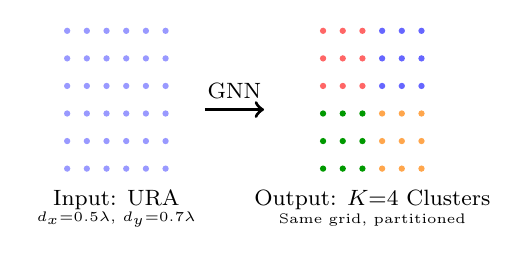
\begin{tikzpicture}[scale=0.5]
    % Input: Regular grid with asymmetric spacing
    \begin{scope}[xshift=0cm]
        \foreach \x in {0,1,2,3,4,5} {
            \foreach \y in {0,1,2,3,4,5} {
                \fill[blue!40] (\x*0.5, \y*0.7) circle (0.08);
            }
        }
        \node[font=\footnotesize] at (1.25, -0.8) {Input: URA};
        \node[font=\tiny] at (1.25, -1.3) {$d_x{=}0.5\lambda$, $d_y{=}0.7\lambda$};
    \end{scope}
    
    % Arrow
    \draw[->, very thick] (3.5, 1.5) -- (5, 1.5) node[midway, above, font=\footnotesize] {GNN};
    
    % Output: Clustered grid (asymmetric)
    \begin{scope}[xshift=6.5cm]
        \foreach \x in {0,1,2} {
            \foreach \y in {3,4,5} {
                \fill[red!60] (\x*0.5, \y*0.7) circle (0.08);
            }
        }
        \foreach \x in {3,4,5} {
            \foreach \y in {3,4,5} {
                \fill[blue!60] (\x*0.5, \y*0.7) circle (0.08);
            }
        }
        \foreach \x in {0,1,2} {
            \foreach \y in {0,1,2} {
                \fill[green!60!black] (\x*0.5, \y*0.7) circle (0.08);
            }
        }
        \foreach \x in {3,4,5} {
            \foreach \y in {0,1,2} {
                \fill[orange!70] (\x*0.5, \y*0.7) circle (0.08);
            }
        }
        \node[font=\footnotesize] at (1.25, -0.8) {Output: $K{=}4$ Clusters};
        \node[font=\tiny] at (1.25, -1.3) {Same grid, partitioned};
    \end{scope}
\end{tikzpicture}
\end{center}

% ============================================================================
% APPENDIX
% ============================================================================
\appendix
\section{Mathematical Notation Reference}

\begin{table}[h]
\centering
\begin{tabular}{@{}cl@{}}
\toprule
\textbf{Symbol} & \textbf{Meaning} \\
\midrule
\multicolumn{2}{@{}l}{\textit{Array Geometry (Fixed)}} \\
$N = 256$ & Number of antenna elements ($16 \times 16$) \\
$(m, n)$ & Grid indices, $m, n \in \{0, 1, \ldots, 15\}$ \\
$d_x = 0.5\lambda$ & Horizontal inter-element spacing \\
$d_y = 0.7\lambda$ & Vertical inter-element spacing \\
$\lambda$ & Wavelength at operating frequency \\
$\mathbf{p}_{m,n} = (m \cdot 0.5\lambda, n \cdot 0.7\lambda)$ & Physical position of element $(m,n)$ \\
\midrule
\multicolumn{2}{@{}l}{\textit{Graph Structure}} \\
$\mathcal{G} = (\mathcal{V}, \mathcal{E})$ & Graph (vertices, edges) \\
$\mathbf{A} \in \mathbb{R}^{N \times N}$ & Adjacency matrix \\
$\mathbf{D} \in \mathbb{R}^{N \times N}$ & Degree matrix (diagonal) \\
$\mathcal{N}(i)$ & Neighbors of node $i$ (4 or 8 connected) \\
\midrule
\multicolumn{2}{@{}l}{\textit{Features}} \\
$\mathbf{x}_i \in \mathbb{R}^d$ & Node feature vector (position) \\
$\mathbf{e}_{ij} = (\Delta x, \Delta y, r)$ & Edge features (physical offsets in $\lambda$) \\
$M_{ij}$ & Mutual coupling between elements $i$ and $j$ \\
\midrule
\multicolumn{2}{@{}l}{\textit{GNN Variables}} \\
$\mathbf{h}_i^{(\ell)} \in \mathbb{R}^{d_\ell}$ & Embedding of node $i$ at layer $\ell$ \\
$\alpha_{ij}$ & Attention weight from $j$ to $i$ \\
$\mathbf{W}^{(\ell)}$ & Learnable weight matrix at layer $\ell$ \\
\midrule
\multicolumn{2}{@{}l}{\textit{Clustering Output}} \\
$K$ & Number of clusters \\
$\mathbf{Z} \in \mathbb{R}^{N \times K}$ & Soft cluster assignment matrix \\
$z_{ik}$ & Probability: node $i$ in cluster $k$ \\
$c_i \in \{1, \ldots, K\}$ & Hard cluster assignment for node $i$ \\
\bottomrule
\end{tabular}
\end{table}

\section{Troubleshooting Common Issues}

\begin{enumerate}
    \item \textbf{All nodes assigned to one cluster:}
    \begin{itemize}
        \item Increase $\lambda_1$ (orthogonality weight)
        \item Add entropy regularization
        \item Check if learning rate is too high
    \end{itemize}
    
    \item \textbf{Very unbalanced clusters:}
    \begin{itemize}
        \item Increase orthogonality loss weight
        \item Try different $k$ for graph construction
    \end{itemize}
    
    \item \textbf{Loss not decreasing:}
    \begin{itemize}
        \item Reduce learning rate
        \item Check for NaN in gradients
        \item Normalize input positions
    \end{itemize}
    
    \item \textbf{Clusters don't respect spatial proximity:}
    \begin{itemize}
        \item Increase $k$ in $k$-NN
        \item Add more GNN layers
        \item Use edge features (distance)
    \end{itemize}
\end{enumerate}

\end{document}